\documentclass{beamer}
\usepackage[authordate,backend=biber]{biblatex-chicago}
\usepackage{xcolor}
\usepackage{soul}
\renewcommand*{\bibfont}{\normalfont\scriptsize}
\makeatletter
\let\HL\hl
\renewcommand\hl{%
  \let\set@color\beamerorig@set@color
  \let\reset@color\beamerorig@reset@color
  \HL}
\makeatother
\addbibresource{2023-05_Presentation.bib}
\usetheme{CambridgeUS}
\usecolortheme{spruce}
\usepackage{graphicx}
\usepackage{longtable,booktabs,array}
\AtBeginSection[]
{
  \begin{frame}
    \frametitle{Table of Contents}
    \tableofcontents[currentsection]
  \end{frame}
}
%Information to be included in the title page:
\title{Land Use Restrictions and Segregation
}
\subtitle{The Effect of Single-Family Zoning in Austin}
\author{Noah J. Case}
\institute{Vassar College}
\date{May 3, 2023}

\begin{document}

\frame{\titlepage}

\section{Introduction}

\begin{frame}{Background}
    \begin{itemize}
        \item Expenditures on housing make up more than one-third of annual consumer spending in the United States (Bureau of Labor Statistics 2022, Table B).
        
        \item Blacks and Hispanics spend an even higher proportion of their incomes on housing than do Whites, despite being likelier to live in multi-family housing (Harvard JCHS 2017; Harvard JCHS 2011)
        
        \item Many point to zoning as a cause of high housing costs, because it diminishes the available quantity of housing (Quigley and Raphael
        2004, page 205).
        
        \item Zoning has macroeconomic consequences, because it channels economic activity further from centers of agglomeration (Hsieh and Moretti 2019).
    \end{itemize}
\end{frame}

\begin{frame}{Research Questions}
    \begin{itemize}
        \item Does single-family zoning cause segregation?
        \item What is the mechanism? People of color are poorer than Whites, but does that explain racial segregation?
        \item Are there heterogeneities in the relationship between zoning and segregation?
        \item How segregated would US cities be without zoning?
    \end{itemize}
\end{frame}

\begin{frame}{Hypothesis}
    Single-Family zoning causes segregation by diminishing the quantity of housing available.
    \begin{itemize}
        \item Zoning is the set of laws and regulations that determine what type of housing can be built and in what quantities. Zoning varies within and across cities. I study variation in zoning within one city.
        \item Segregation, for my purposes, is when there are significant differences in the racial composition of adjacent census blocks on either side of a zoning boundary.
        \item Zoning functions as a decrease in housing supply.
        \item I explore various mechanisms, such as income, preferences, and signalling.
    \end{itemize} 
\end{frame}

\section{Literature Review}

\begin{frame}{Zoning Literature}
    \begin{itemize}
        \item Seminal Coase (1960) paper on externalities.
        \begin{itemize}
            \item Externalities are resolved if there are complete property rights and frictionless bargaining.
        \end{itemize}
        \item Fischel (1975) book \textit{The Economics of Zoning Laws}.
        \begin{itemize}
            \item Zoning is an incomplete assignment of property rights, so the externalities are not resolved.
        \end{itemize}
        \item Resseger (2022) paper on zoning and segregation in Boston.
        \begin{itemize}
            \item Permitting multi-family housing by right increases integration.
        \end{itemize}
    \end{itemize}
\end{frame}

\begin{frame}[allowframebreaks]{Measuring Segregation}
    I take advantage of the rich literature of nuanced segregation measures:
    \begin{itemize}
        \item Herfindal-Hirshman Index (1950)

        \begin{equation}
    \text{HHI}=\sum_{i=1}^n \left(\frac{\text{Population}_i}{\text{Population}}\right)^2
\end{equation}

        \item Dissimilarity Index (Jahn, Schmid, and Schrag 1947)

        \begin{equation}
    D=\frac{1}{2}\sum_{i=1}^N\left|\frac{\text{White}_i}{\text{White}_{total}}-\frac{\text{non-White}_i}{\text{non-White}_{total}}\right|
\end{equation}
\framebreak
        \item Exposure Index (Blau 1977)

        \begin{equation}
    E=\sum_{i=1}^n\left(\frac{\text{non-White}_i}{\text{non-White}_{total}}\right)\left(\frac{\text{White}_i}{\text{Population}_{i}}\right)
\end{equation}

        \item Entropy Index (White 1986)

        \begin{equation}
    H=-\sum_{i=1}^n\text{share}_i \log(\text{share}_i)
\end{equation}
    \end{itemize}
\end{frame}

\section{Empirical Strategy}

\begin{frame}{Data}
\begin{itemize}
    \item I use demographic data from the US census for income and race at the census tract- and block-level respectively.
    \item I use by-address zoning data for all Austin addresses.
    \item I use the Census Bureau's free batch geocoder service to match addresses to census blocks.
    \item This allows me to construct a dataset of race, zoning, and income by census block in Austin.
    \end{itemize}
\end{frame}
\begin{frame}{Identification}
    \begin{itemize}
        \item I identify the causal effect of zoning on racial makeup by selecting census blocks adjacent to zoning boundaries in Austin, TX.
        \item This method builds on Resseger (2022) who used a similar method to estimate the segregating effect of zoning in and around Boston, MA.
    \end{itemize}
\end{frame}

\begin{frame}{Map of Austin Census Blocks}
    \begin{figure}
    \centering
    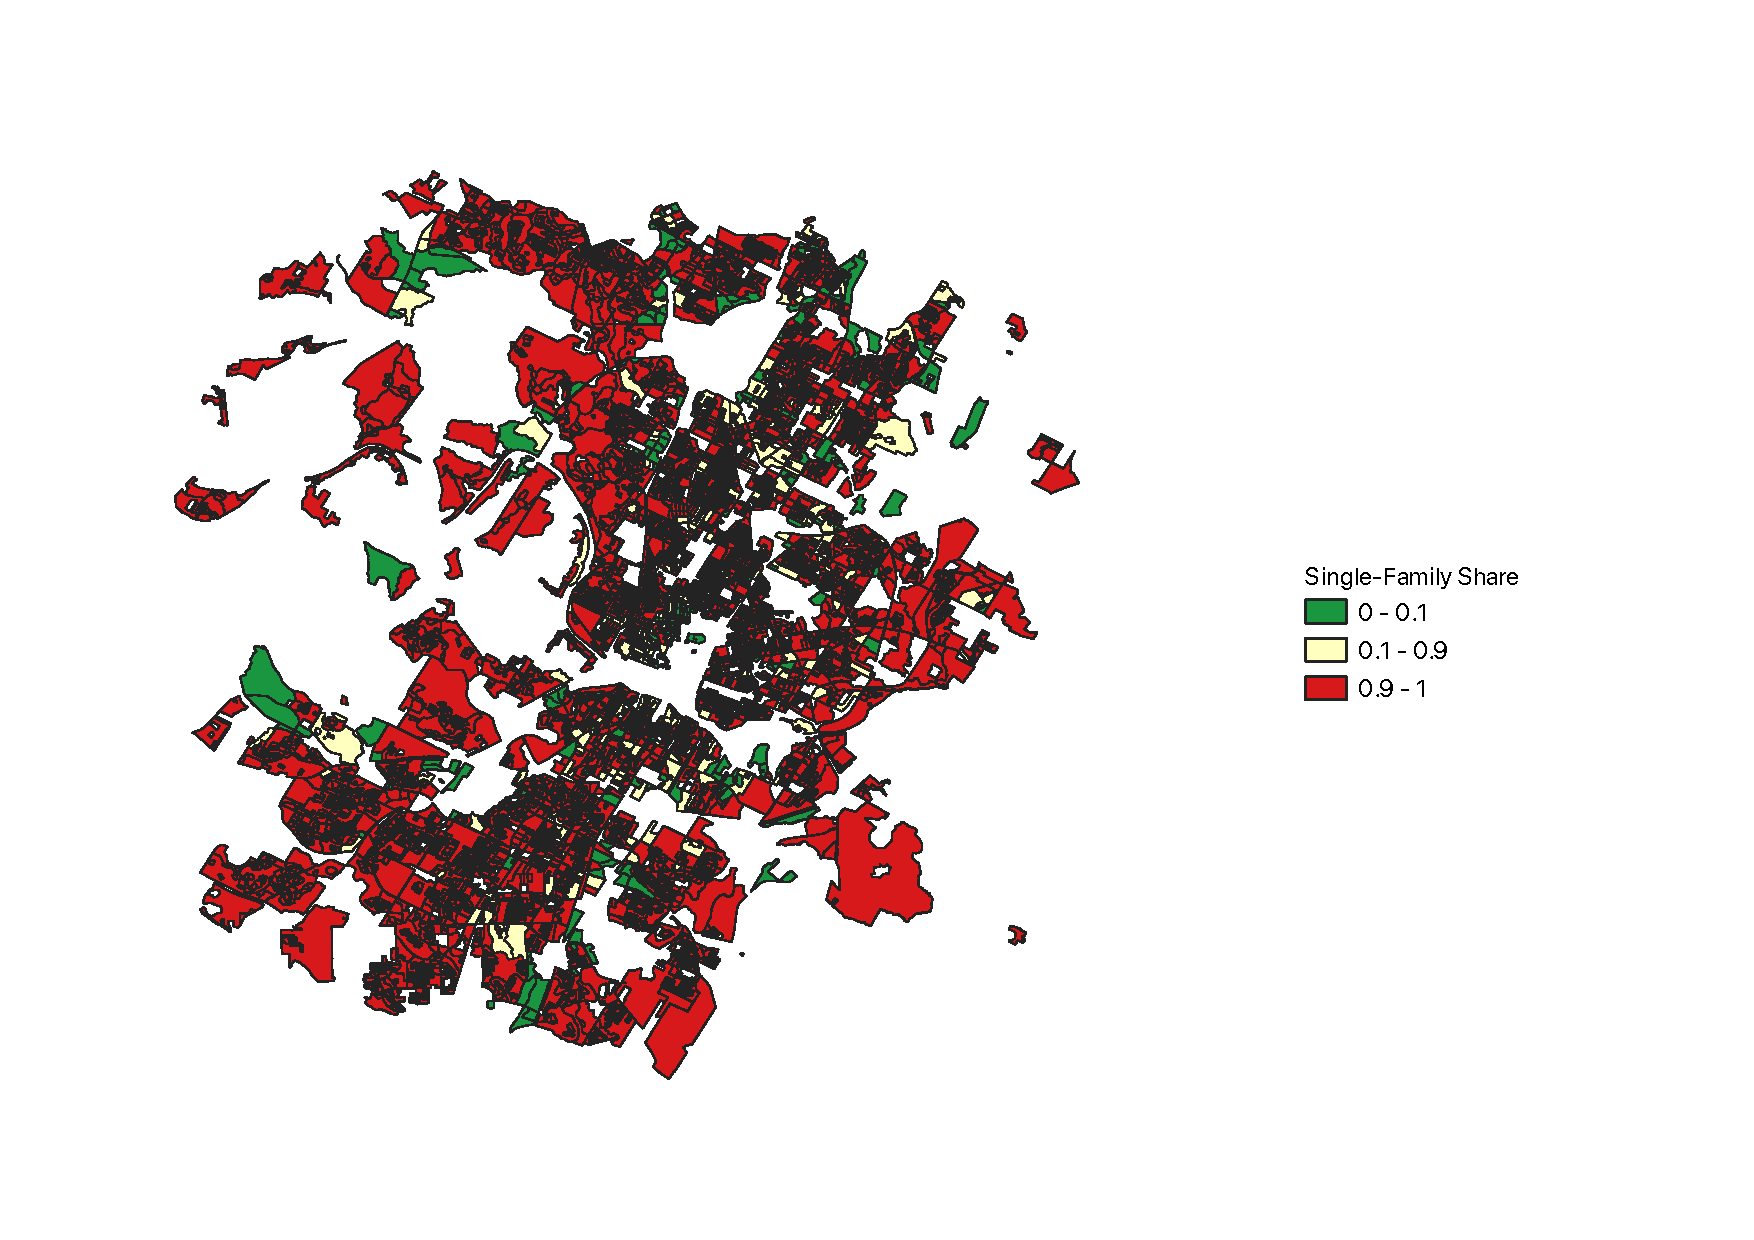
\includegraphics[width=\textwidth]{fig1_redone_output.pdf}
    \caption{Map of Austin Census Blocks Colored by Zoning}
    \label{fig:Austin_Zoning_Map}
\end{figure}
\end{frame}

\begin{frame}{Boundary Subset}
    \begin{figure}[h]
    \centering
    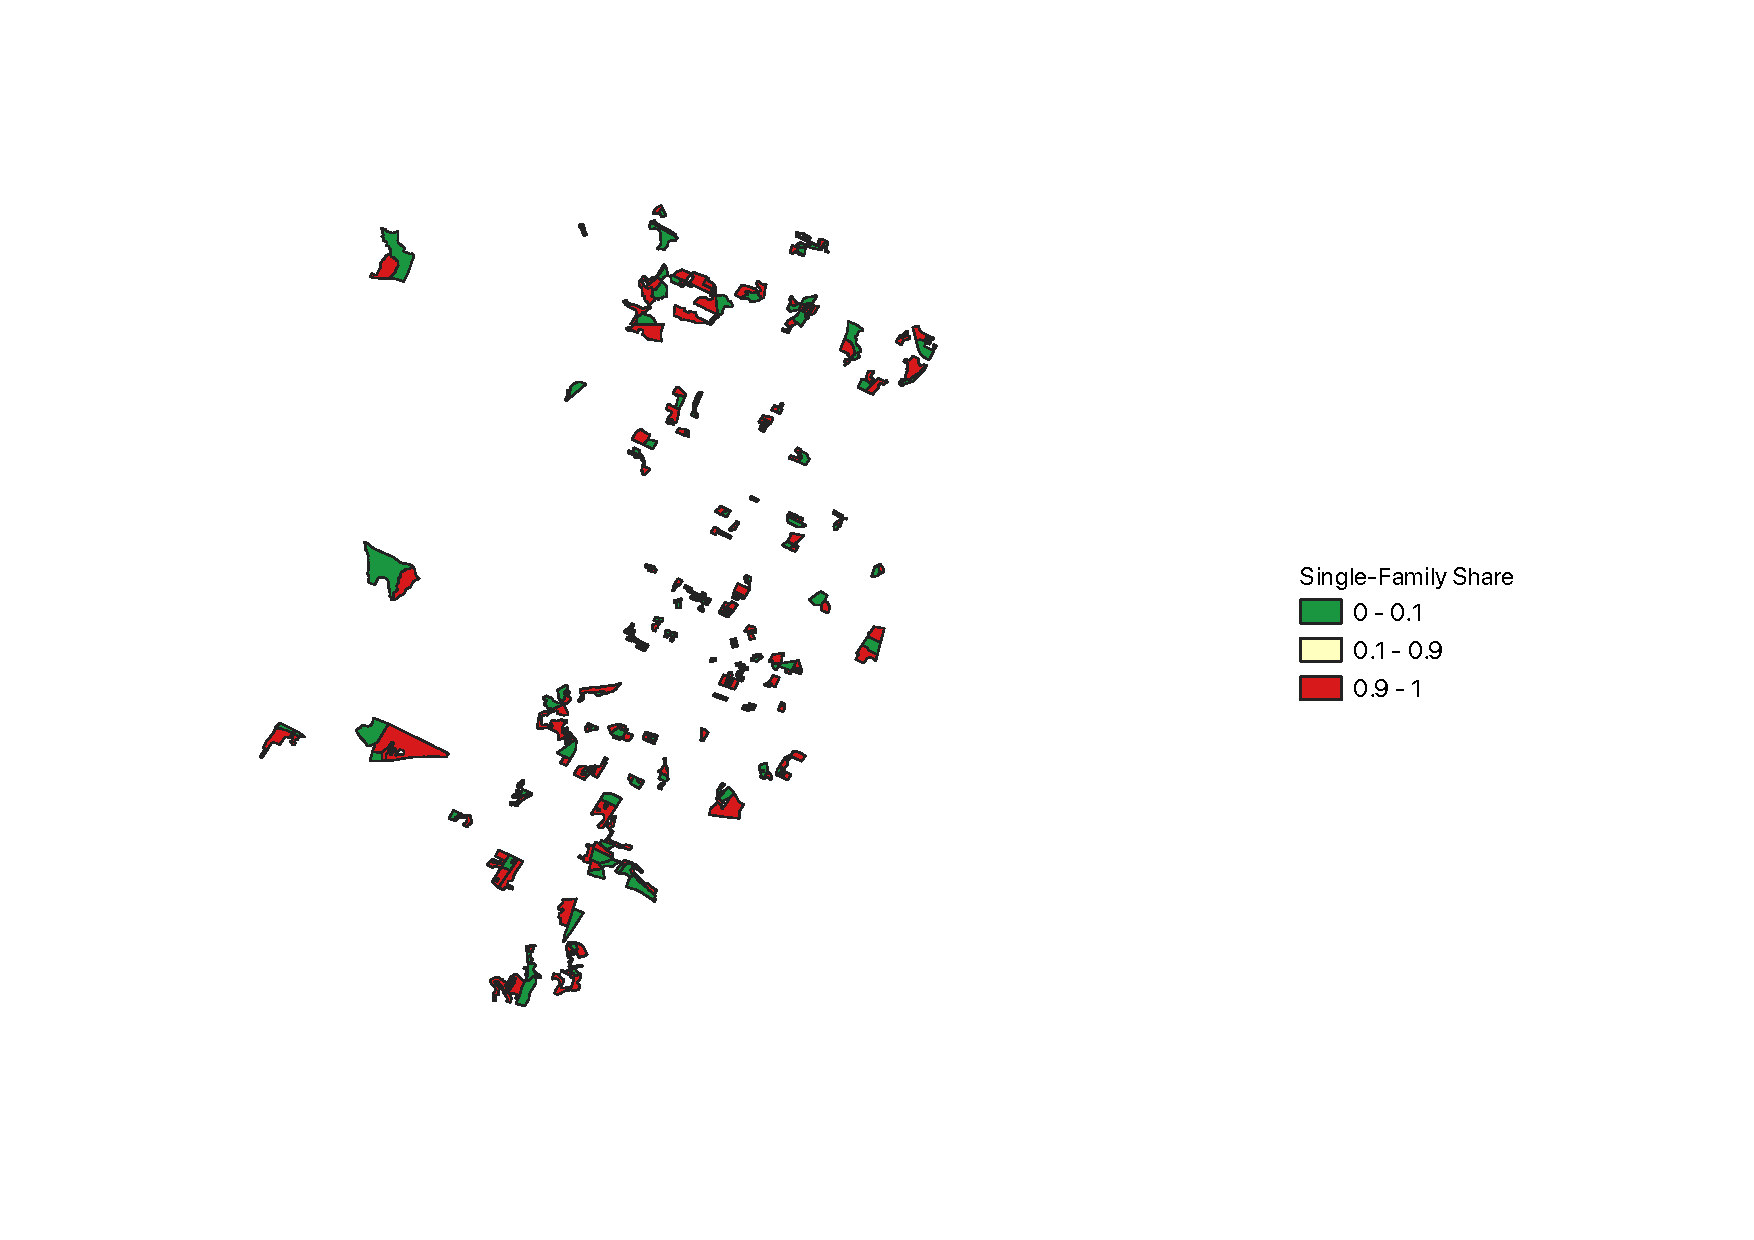
\includegraphics[width=\textwidth]{fig_2_causal_redone.pdf}
    \caption{Map of Boundary Subset of Census Blocks}
    \label{fig:Causal_Map}
\end{figure}
\end{frame}

\begin{frame}{Summary Statistics}

\begin{table}
\footnotesize
\caption{Summary Statistics for Boundary Subset (N=332)}
\\[1.8ex]
\label{tab:causal_summary_stats}
\centering
\begin{tabular}[!htbp]{@{\extracolsep{5pt}}lccccc} 
\hline
\hline
\\[-1.8ex] 
Variables & Mean & Median & SD & Min & Max\\
\\[-1.8ex] \hline\\[-1.8ex] 
Population & 228.401 & 94.000 & 324.142 & 3.000 & 2152.000 \\

Share Non-Hispanic-White & 0.505 & 0.521 & 0.236 & 0.000 & 0.949 \\

Share Black & 0.085 & 0.046 & 0.120 & 0.000 & 0.767 \\

Share Asian & 0.067 & 0.039 & 0.095 & 0.000 & 0.782 \\

Share AIAN & 0.012 & 0.000 & 0.029 & 0.000 & 0.263 \\

Share NHPI & 0.001 & 0.000 & 0.009 & 0.000 & 0.125 \\

Share Other & 0.100 & 0.069 & 0.110 & 0.000 & 0.562 \\

Share Multiracial & 0.159 & 0.135 & 0.107 & 0.000 & 0.875 \\

Share Hispanic & 0.288 & 0.235 & 0.189 & 0.000 & 0.895 \\

Median Household Income & 71,150 & 71,467 & 25,912 & 6322 & 228,929\\

SF-Zoned Addresses & 0.597 & 0.972 & 0.483 & 0.000 & 1.000 \\

HHI & 4655 & 4399 & 1447 & 1562 & 9007 \\
Entropy Index & 0.893 & 0.918 & 0.247 & 0.144 & 1.451 \\
\hline
\hline
\end{tabular}
\end{table}
\end{frame}

\begin{frame}{Limitations}
    \begin{itemize}
        \item Multi-family addresses are twice as likely to have no match when I geocode.
        \item Local Average Treatment Effect problem, similar to other discontinuity designs.
        \item Generalizability.
        \item Residual Endogeneity.
    \end{itemize}
\end{frame}

\section{Results}

\begin{frame}{Bivariate Regressions over the Boundary Subset}
    I regress the white share in each census block on zoning in a naive bivariate regression, first with OLS, and then with Logistic Regression.
    
    \begin{equation} \label{biv_regression}
        Y_i=\alpha+\beta S_i+\epsilon_i
    \end{equation}
    
    \begin{equation}
        Z_i=\log\left(\frac{Y_i}{1-Y_i}\right)
    \end{equation}
\end{frame}

\begin{frame}{Results from Bivariate Regressions}
\footnotesize
\begin{table}[!htbp] \centering 
  \caption{Bivariate Regressions, Geographic Discontinuity Design} 
  \label{tab:naive_biv_causal} 
\begin{tabular}{@{\extracolsep{5pt}}lcc} 
\\[-1.8ex]\hline 
\hline \\[-1.8ex] 
 & \multicolumn{2}{c}{\textit{Dependent variable:}} \\ 
\cline{2-3} 
\\[-1.8ex] & \multicolumn{2}{c}{White Share} \\ 
\\[-1.8ex] & \textit{OLS} & \textit{Logistic} \\ 
\\[-1.8ex] & (1) & (2)\\ 
\hline \\[-1.8ex] 
 Single Family Share & \hl{0.082$^{***}$} & 0.329$^{***}$ \\ 
  & (0.026) & (0.106) \\ 
  & & \\ 
\hline \\[-1.8ex] 
Observations & 332 & 332 \\ 
Adjusted R$^{2}$ & 0.025 &  \\ 
Log Likelihood &  & $-$227.197 \\ 
\hline 
\hline \\[-1.8ex] 
 \multicolumn{3}{r}{\textit{Note}: Robust Standard Errors in Parentheses. $^{*}$p$<$0.1; $^{**}$p$<$0.05; $^{***}$p$<$0.01} \\ 
\end{tabular} 
\end{table} 
\end{frame}

\begin{frame}{Regressions with Controls}
    I repeat the regression from the previous slide with controls for block population $P_i$, neighborhood characteristics (Census Tract FE) $\boldsymbol{B_a}$, and census tract income, $W_a$. I use OLS and Logistic specifications, but focus on the OLS models.

    \begin{equation} \label{eqn:full_model_income}
    Y_{ia}=\alpha+\beta S_i+\delta P_i+\varphi W_a +\epsilon_{ia}
    \end{equation}

    \begin{equation} \label{eqn:full_model_FEs}
    Y_{ia}=\alpha+\beta S_i+\delta P_i+\boldsymbol{\gamma}\cdot\boldsymbol{B_a} +\epsilon_{ia}
    \end{equation}
    
\end{frame}

\begin{frame}{OLS Results with Controls}
\footnotesize
\begin{table}[!htbp] \centering 
  \caption{OLS Estimates with Controls,  Geographic Discontinuity Design}
  \label{tab:OLS_controls_causal} 
\begin{tabular}{@{\extracolsep{5pt}}lccccc} 
\\[-1.8ex]\hline 
\hline \\[-1.8ex] 
 & \multicolumn{5}{c}{\textit{Dependent variable:}} \\ 
\cline{2-6} 
\\[-1.8ex] & \multicolumn{5}{c}{White Share} \\ 
\\[-1.8ex] & (1) & (2) & (3) & (4) & (5)\\ 
\hline \\[-1.8ex] 
 Single Family Share & 0.073$^{***}$ & 0.071$^{***}$ & 0.085$^{***}$ & \hl{0.087$^{***}$} & 0.066$^{**}$ \\ 
  & (0.026) & (0.027) & (0.025) & (0.026) & (0.027) \\ 
  & & & & & \\ 
\hline \\[-1.8ex] 
Observations & 332 & 332 & 332 & 332 & 332 \\ 
Adjusted R$^{2}$ & 0.079 & 0.029 & 0.429 & 0.427 & 0.080 \\ 
\hline
Income & Y & N & N & N & Y\\
Population & N & Y & N & Y & Y\\
Tract FE & N & N & Y & Y & N\\
\hline 
\hline \\[-1.8ex] 
\multicolumn{6}{l}{\textit{Note:} Robust Standard Errors in Parentheses. $^{*}$p$<$0.1; $^{**}$p$<$0.05; $^{***}$p$<$0.01} \\ 
\end{tabular} 
\end{table}
\end{frame}

\section{Discussion}

\begin{frame}{Mechanisms}
    \begin{itemize}
        \item Income: I show that the relationship between zoning and segregation survives various controls for income.
        
        \item Preferences: The Schelling (1971) model of segregation suggests that even small racial differences in housing preference can lead to segregation, but DeFina (2007) studies this empirically and finds no strong evidence.
        
        \item Self-Segregating: Some scholars have suggested that Blacks have a particular and idiosyncratic preference for self-segregation. The empirical evidence for this is weak.

        \item Signalling: Zoning is a signal of the likelihood a non-White resident will experience discriminatory treatment in a particular neighborhood.       
    \end{itemize}
\end{frame}

\begin{frame}{Heterogeneity}
\begin{itemize}
    \item Geographic: I test for heterogeneous effects north and south of the Colorado River, and find no significant heterogeneity.

    \item Class: I test for heterogeneous effects in the rich half of the sample, and again find no significant heterogeneity.
\end{itemize}
\end{frame}

\begin{frame}{Robustness}
    I use a weighted regression on the boundary subset, where I weigh tighter spatial comparisons more strongly. Coefficients on zoning continue to be significant and socially meaningful, suggesting that my results are \textit{not} driven by poor spatial comparisons.
\end{frame}

\begin{frame}{Policy Implications}
    \begin{itemize}
        \item My results indicate that zoning causes racial segregation. This means governments can promote integration by liberalizing zoning. 

        \item The politics of this reform are challenging, but not impossible. The traditional opponents of zoning reform are incumbent homeowners. But broad-based upzoning increase property values by increasing the property rights associated with land ownership.

        \item Options for reforms: I focus on single- versus multi-family, but FAR, setback requirements, building codes, etc. also offer avenues for reform.
    \end{itemize}  
\end{frame}

\begin{frame}{Concluding Remarks}
    \begin{itemize}
        \item I find that a one standard deviation increase (25.7 percentage points) in single-family zoning causes a census block to have 2.2 percentage points more white people.
        
        \item This result holds even when I use more sophisticated measures of segregation, such as the Entropy and Herfindahl-Hirshman Indices.

        \item Future research should try to replicate these results in different cities, particularly as more data becomes available.

        \item And, as empirical estimates of zoning's effects become more reliable and abundant, the next step is identifying mechanisms.
    \end{itemize}
\end{frame}

\section*{References}

\begin{frame}[allowframebreaks]{References}
\footnotesize
    \nocite{*}
\printbibliography[heading=none]
\end{frame}

\section*{Appendix Tables}

\begin{frame}{Heterogeneity Tables}
    \tiny
    \begin{table}[!htbp] \centering 
  \caption{Test for Heterogeneous Effects by Census Tract Income} 
  \label{tab:income_heterogeneity} 
\begin{tabular}{@{\extracolsep{5pt}}lcc} 
\\[-1.8ex]\hline 
\hline \\[-1.8ex] 
 & \multicolumn{2}{c}{\textit{Dependent variable:}} \\ 
\cline{2-3} 
\\[-1.8ex] & \multicolumn{2}{c}{White Share} \\ 
\\[-1.8ex] & \textit{OLS} & \textit{Logistic} \\ 
\\[-1.8ex] & (1) & (2)\\ 
\hline \\[-1.8ex] 
 Single Family Share & 0.073$^{**}$ & 0.326 \\ 
  & (0.032) & (0.383) \\ 
  & & \\ 
 Single Family Share $\times$ Rich Indicator & 0.028 & 0.139 \\ 
  & (0.046) & (0.548) \\ 
  & & \\ 
\hline \\[-1.8ex] 
Observations & 332 & 332 \\ 
Adjusted R$^{2}$ & 0.425 &  \\ 
Log Likelihood &  & $-$166.228 \\ 
Akaike Inf. Crit. &  & 534.457 \\ 
\hline 
\hline \\[-1.8ex] 
\textit{Note:} Robust Standard Errors in Parentheses.  & \multicolumn{2}{r}{$^{*}$p$<$0.1; $^{**}$p$<$0.05; $^{***}$p$<$0.01} \\ 
\end{tabular} 
\end{table} 
\end{frame}

\begin{frame}{Heterogeneity Tables}
    \tiny
\begin{table}[H] \centering 
  \caption{Test for Heterogeneous Effects in North vs. South Austin} 
  \label{tab:river_heteroeneity} 
\begin{tabular}{@{\extracolsep{5pt}}lcc} 
\\[-1.8ex]\hline 
\hline \\[-1.8ex] 
 & \multicolumn{2}{c}{\textit{Dependent variable:}} \\ 
\cline{2-3} 
\\[-1.8ex] & \multicolumn{2}{c}{White Share} \\ 
\\[-1.8ex] & \textit{OLS} & \textit{Logistic} \\ 
\\[-1.8ex] & (1) & (2)\\ 
\hline \\[-1.8ex] 
 Single Family Share & 0.101$^{**}$ & 0.444 \\ 
  & (0.042) & (0.499) \\ 
  & & \\ 
 Single Family Share $\times$ North Indicator & $-$0.021 & $-$0.075 \\ 
  & (0.050) & (0.591) \\ 
  & & \\ 
\hline \\[-1.8ex] 
Observations & 332 & 332 \\ 
Adjusted R$^{2}$ & 0.425 &  \\ 
Log Likelihood &  & $-$166.455 \\ 
Akaike Inf. Crit. &  & 534.910 \\ 
\hline 
\hline \\[-1.8ex] 
\textit{Note:} Robust Standard Errors in Parentheses  & \multicolumn{2}{r}{$^{*}$p$<$0.1; $^{**}$p$<$0.05; $^{***}$p$<$0.01} \\ 
\end{tabular} 
\end{table}
\end{frame}

\begin{frame}{Entropy Table}
\tiny
\begin{table}[!htbp] \centering 

  \caption{Regressions on the Entropy Index, Boundary Subset} 
  \label{tab:Entropy_Causal} 
\begin{tabular}{@{\extracolsep{5pt}}lccccc} 
\\[-1.8ex]\hline 
\hline \\[-1.8ex] 
 & \multicolumn{5}{c}{\textit{Dependent variable:}} \\ 
\cline{2-6} 
\\[-1.8ex] & \multicolumn{5}{c}{Entropy Index} \\ 
\\[-1.8ex] & (1) & (2) & (3) & (4) & (5)\\ 
\hline \\[-1.8ex] 
 Single Family Share & $-$0.093$^{***}$ & $-$0.066$^{**}$ & $-$0.094$^{***}$ & \hl{$-$0.076$^{***}$} & $-$0.061$^{**}$ \\ 
  & (0.027) & (0.027) & (0.026) & (0.027) & (0.027) \\ 
  & & & & & \\ 
\hline \\[-1.8ex] 
Observations & 332 & 332 & 332 & 332 & 332 \\ 
Adjusted R$^{2}$ & 0.092 & 0.101 & 0.297 & 0.312 & 0.144 \\ 
\hline
Income Control & Y & N & N & N & Y\\
Population Control & N & Y & N & Y & Y\\
Tract FE & N & N & Y & Y & N\\
\hline 
\hline \\[-1.8ex] 
\multicolumn{6}{l}{\textit{Note:} Robust Standard Errors in Parentheses. $^{*}$p$<$0.1; $^{**}$p$<$0.05; $^{***}$p$<$0.01} \\
\end{tabular} 
\end{table} 

    
\end{frame}

\begin{frame}{HHI Table}
    \tiny
    \begin{table}[!htbp] \centering 
  \caption{Regressions on the Herfindahl-Hirschman Index, Boundary Subset} 
  \label{tab:HHI_Causal} 
\begin{tabular}{@{\extracolsep{5pt}}lccccc} 
\\[-1.8ex]\hline 
\hline \\[-1.8ex] 
 & \multicolumn{5}{c}{\textit{Dependent variable:}} \\ 
\cline{2-6} 
\\[-1.8ex] & \multicolumn{5}{c}{Herfindahl-Hirschman Index} \\ 
\\[-1.8ex] & (1) & (2) & (3) & (4) & (5)\\ 
\hline \\[-1.8ex] 
 Single Family Share & 478.664$^{***}$ & 408.978$^{**}$ & 526.791$^{***}$ & \hl{498.155$^{***}$} & 384.016$^{**}$ \\ 
  & (157.522) & (162.471) & (161.051) & (166.120) & (161.007) \\ 
  & & & & & \\ 
\hline \\[-1.8ex] 
Observations & 332 & 332 & 332 & 332 & 332 \\ 
Adjusted R$^{2}$ & 0.061 & 0.043 & 0.210 & 0.208 & 0.072 \\ 
\hline
Income Control & Y & N & N & N & Y\\
Population Control & N & Y & N & Y & Y\\
Tract FE & N & N & Y & Y & N\\
\hline 
\hline \\[-1.8ex] 
\multicolumn{6}{l}{\textit{Note:} Robust Standard Errors in Parentheses. $^{*}$p$<$0.1; $^{**}$p$<$0.05; $^{***}$p$<$0.01} \\
\end{tabular} 
\end{table} 
\end{frame}

\begin{frame}{Logistic Estimates}
\tiny

\begin{table}[!htbp] \centering 
  \caption{Logistic Estimates with Controls, Boundary Subset} 
  \label{tab:logit_controls_causal} 
\begin{tabular}{@{\extracolsep{5pt}}lccccc} 
\\[-1.8ex]\hline 
\hline \\[-1.8ex] 
 & \multicolumn{5}{c}{\textit{Dependent variable:}} \\ 
\cline{2-6} 
\\[-1.8ex] & \multicolumn{5}{c}{White Share} \\ 
\\[-1.8ex] & (1) & (2) & (3) & (4) & (5)\\ 
\hline \\[-1.8ex] 
 Single Family Share & 0.295$^{***}$ & 0.285$^{***}$ & 0.386$^{***}$ & \hl{0.392$^{***}$} & 0.267$^{**}$ \\ 
  & (0.106) & (0.111) & (0.112) & (0.119) & (0.111) \\ 
  & & & & & \\ 
\hline \\[-1.8ex] 
Observations & 332 & 332 & 332 & 332 & 332\\ 
Log Likelihood & $-$221.291 & $-$226.566 & $-$166.434 & $-$166.433 & $-$221.018 \\ 
Akaike Inf. Crit. & 448.583 & 459.131 & 530.868 & 532.865 & 450.035 \\ 
\hline
Income & Y & N & N & N & Y\\
Population & N & Y & N & Y & Y\\
Tract FE & N & N & Y & Y & N\\
\hline 
\hline \\[-1.8ex] 
\multicolumn{6}{l}{\textit{Note:} Robust Standard Errors in Parentheses. $^{*}$p$<$0.1; $^{**}$p$<$0.05; $^{***}$p$<$0.01} \\
\end{tabular} 
\end{table} 
    
\end{frame}

\begin{frame}{Whole City Estimates}
    \tiny
    \begin{table}[!htbp] \centering 
  \caption{OLS Estimates with Controls} 
  \label{tab:OLS_controls} 
\begin{tabular}{@{\extracolsep{5pt}}lccccc} 
\\[-1.8ex]\hline 
\hline \\[-1.8ex] 
 & \multicolumn{5}{c}{\textit{Dependent variable:}} \\ 
\cline{2-6} 
\\[-1.8ex] & \multicolumn{5}{c}{White Share} \\ 
\\[-1.8ex] & (1) & (2) & (3) & (4) & (5)\\ 
\hline \\[-1.8ex] 
     Single Family Share & 0.026$^{**}$ & 0.055$^{***}$ & 0.095$^{***}$ & \hl{0.091$^{***}$} & $-$0.008 \\ 
  & (0.012) & (0.013) & (0.012) & (0.012) & (0.013) \\ 
  & & & & & \\ 
\hline \\[-1.8ex] 
Observations & 6,250 & 6,252 & 6,252 & 6,252 & 6,250 \\ 
Adjusted R$^{2}$ & 0.142 & 0.023 & 0.602 & 0.602 & 0.151 \\ 
\hline
Income & Y & N & N & N & Y\\
Population & N & Y & N & Y & Y\\
Tract FE & N & N & Y & Y & N\\
\hline 
\hline \\[-1.8ex] 
\multicolumn{6}{l}{\textit{Note:} Robust Standard Errors in Parentheses. $^{*}$p$<$0.1; $^{**}$p$<$0.05; $^{***}$p$<$0.01} \\ 
\end{tabular} 
\end{table}
\end{frame}

\end{document}
